%%%%%%%%%%%%%%%%%%%%%%%%%%%%%%%%%%%%%%%%%%%%%%%%%%%
%% P3: Phenomenology of Particle Physics                         
%%
%% Author:  André Rubbia                   		 
%%
%% Figure 28.4 (left) Illustration of the neutrino flux in a narrow band beam. 
%% (right) Simulated correlation between the radial position and the neutrino energy
%%
%% This work is licensed under the Creative Commons Attribution 4.0 International License. 
%% To view a copy of this license, visit http://creativecommons.org/licenses/by/4.0/ or 
%% send a letter to Creative Commons, PO Box 1866, Mountain View, CA 94042, USA.
%%
%%%%%%%%%%%%%%%%%%%%%%%%%%%%%%%%%%%%%%%%%%%%%%%%%%%

\documentclass[a4paper,10pt]{article}

\usepackage[T1]{fontenc}
\usepackage[utf8]{inputenc}
\usepackage{lmodern}
\usepackage[labelfont=bf]{caption}
\usepackage{upgreek}

\usepackage{listings}

\usepackage{tikz}
\usepackage{pgfplots}
\pgfplotsset{compat=1.17}
\usepgfplotslibrary{ternary}
\usepgfplotslibrary{fillbetween}
\usepgfplotslibrary{external}

\def\d{\mathrm{d}}
\setlength{\oddsidemargin}{-1.0cm}
\setlength{\evensidemargin}{-1.0cm}
\setlength{\textheight}{25cm}
\setlength{\textwidth}{18cm}

\pgfkeys{/pgf/number format/.cd,1000 sep={}}

\begin{document}

%%%%%%%%%%%%%%%%   FIGURE  %%%%%%%%%%%%%%%%%%%%%%%%%%%%%%
\begin{figure}[htb]
\centering
\begin{tikzpicture}[scale=1.]
\begin{axis}[xmin=0, xmax=1.1,
	height = 0.35\textwidth,
	ymin=0, ymax=1.2,
	title=Neutrino flux in a narrow-band beam,
	xlabel=$E_\nu/E_M$,
	ylabel=$\phi(E_\nu)$ (relative units),
	]
	\addplot[domain=0:0.1,blue,very thick] {1000*x^3};
	\addplot[domain=0.1:0.43,blue,very thick] {1};
	\addplot[domain=0.6:0.95,magenta,very thick] {0.6};
	\addplot[domain=0.4:0.6,magenta,very thick] {600*((x-0.4)/2)^3};
	\draw[blue, very thick] (axis cs:0.43,1) -- (axis cs:0.43,0);
	\draw[magenta, very thick] (axis cs:0.95,0.6) -- (axis cs:0.95,0);
	\node[above,blue] at (axis cs:0.25,1) {$\nu_\pi$};
	\node[above,magenta] at (axis cs:0.85,0.6) {$\nu_K$};
\end{axis}
\end{tikzpicture}
\hspace{5mm}
\begin{tikzpicture}[scale=1.]
\begin{axis}[
	height = 0.35\textwidth,
	xmin=0, xmax=300,
	ymin=0, ymax=3,
	title={$p_0 = 300 \pm 5\%$ GeV},
	xlabel=$E_\nu$ (GeV),
	ylabel=$R$ (m),
	]
 \addplot+[only marks, blue, mark=o] table [x=ENU, y=R] {narrowbandbeam.dat};
 \end{axis}
\end{tikzpicture}
\caption{(left) Illustration of the neutrino flux in a narrow band beam.
(right) Simulated correlation between the radial position and the neutrino energy.}
\end{figure}
%
%%%%%%%%%%%%%%%%   END FIGURE  %%%%%%%%%%%%%%%%%%%%%%%%%%%%%%
%

The Python code used to generate the figure on the right is shown below and available on the repository.

\begin{lstlisting}[language=Python]

import random
import math

# distances in meters
# energies in GeV

# mass of particles in GeV
mmuon=105.7e-3
mproton=938.3e-3
mpion=139.570e-3
mkaon=493.677e-3

# beam parameters
# distance to detector (m)
L=800
# momentum selection NBB (GeV)
p0 = 300
# radius of beam (sigma)
r0 = 0.3
# decay tunnel (m)
decaytunnellength = 300
decaytunnelradius = 1

f = open('narrowbandbeam.dat', 'w')

title = "ENU   R\n"
f.write(title)

for i in range(0,100000):

    pbeam = (1+random.gauss(0, 0.05))*p0
    x0 = random.gauss(0,r0)
    y0 = random.gauss(0,r0)
    rbeam = math.sqrt(x0**2+y0**2)
    if(abs(rbeam) > decaytunnelradius):
        continue

# assume 70% of pions in the beam
    if(random.random()<0.7):
        mmeson = mpion
        tau=26e-9
    else:
        mmeson = mkaon
        tau=12e-9

    ebeam = math.sqrt(pbeam**2+mmeson**2)
    beta = pbeam/ebeam
    gamma = ebeam/mmeson

    decaypoint = -gamma*3e8*tau*math.log(random.random())
    if(decaypoint>decaytunnellength):
        continue

    # maximum energy in meson CMS
    enustar = (mmeson**2 - mmuon**2)/(2*mmeson)

    # decay angle in the meson CMS
    costhetastar = random.uniform(-1,1)

    # lab quantities
    enu = gamma*enustar*(1+beta*costhetastar)
    costheta = (costhetastar+beta)/(1+beta*costhetastar)
    sintheta = math.sqrt(1-costheta**2)
    tantheta = sintheta/costheta
    phi = 2*math.pi*random.random()
    x = (L-decaypoint)*tantheta*math.cos(phi)+x0
    y = (L-decaypoint)*tantheta*math.sin(phi)+y0
    R = math.sqrt(x**2+y**2)

    if(R<3):
        out = "%f\t%f\n" % (enu,R)
        f.write(out)

f.close()

\end{lstlisting}

\end{document}
